\documentclass[12pt]{article}
\usepackage{amsgen,amsmath,amstext,amsbsy,amsopn,amssymb}
%\usepackage[dvips]{graphicx,color}
\usepackage{graphicx,color,bm}
\usepackage{epsfig}
\usepackage{enumerate}
\usepackage{float}
\usepackage{multicol}
\usepackage{longtable}
\usepackage{verbatim}
\usepackage{hyperref}
\usepackage[utf8]{inputenc}
\usepackage[english]{babel}
\usepackage{commath}
\usepackage{tikz}
\usepackage{wrapfig,lipsum,booktabs}
\usepackage{subcaption}
%\setlength{\oddsidemargin}{0.1 in} \setlength{\evensidemargin}{-0.1
%in} \setlength{\topmargin}{-0.6 in} \setlength{\textwidth}{6.5 in}
%\setlength{\textheight}{8.5 in} \setlength{\headsep}{0.75 in}
%\setlength{\parindent}{0 in} \setlength{\parskip}{0.1 in}

\textwidth 6.3in \textheight 8.8in \topmargin -0.5truein
\oddsidemargin .15truein
\parskip .1in
\renewcommand{\baselinestretch}{1.00}  % double spaced
\renewcommand{\thesection}{\Roman{section}} 
\renewcommand{\thesubsection}{\thesection.\Roman{subsection}}
\newcommand*{\addheight}[2][.5ex]{%
	\raisebox{0pt}[\dimexpr\height+(#1)\relax]{#2}%
}
\usepackage{caption}

\begin{document}
	
\title{%
	CSE 515 HW 4}

\author{ Alexander Van Roijen}

\maketitle	
\begin{section}{8.1}
	\subsection{A}
	A simple mechanism to sample from this distribution would be to sample uniformly from entries 1...N, and then removing whichever entry was sampled, and then continuing this process until N entries have been selected. Also known as sampling from 1 to N with replacement
	\subsection{B}
	First note that this holds up as in our previous problem, as $\max_{i,j}w_{i,j}=0$ would give us $\frac{1}{N!}$ which is exactly the probability of one sample from $1..N$ that satisfies a perfect matching with a uniform distribution.
	\\
	\begin{gather}
		\mu(\sigma_j) = \frac{1}{Z}\exp(\Sigma_{i}w_{i,\sigma(j,i)})I(\sigma_j = \text{perfect matching})\\
		\rightarrow Z = \Sigma_j \mu(\sigma_j) = \Sigma_j\exp(\Sigma_{i}w_{i,\sigma(j)})N!\\
		\rightarrow Z \le \exp(\Sigma_{i}w^*)N! = \exp(Nw^*)N! \\
		\rightarrow \mu(\sigma_i) = \frac{1}{Z}\exp(\Sigma_{i}w_{i,\sigma(j,i)})I(\sigma_j = \text{perfect matching})  \ge \frac{1}{Z} 
		 =  \frac{1}{\exp(Nw^*)N!}\square
	\end{gather}
	1 is by definition\\
	2 is also by definition\\
	3 by substituting in w* and since the exponential is monotonically increasing\\
	4 as $ \exp(\Sigma_{i}w_{i,\sigma(j,i)}) > 1$ and definition\\
	\subsection{C}
	\begin{gather}
		\exp(w_{i\sigma(i')}+w_{i'\sigma(i)}-w_{i\sigma(i)}-w_{i'\sigma(i')}) = \frac{\exp(w_{i\sigma(i')}+w_{i'\sigma(i)})}{\exp(w_{i\sigma(i)}+w_{i'\sigma(i')})}\\
		\ge \frac{1}{\exp(w_{i\sigma(i)}+w_{i'\sigma(i')})} \text{as } \exp(y)\ge 1 \forall y \ge 0\\
		\ge \frac{1}{\exp(2w^*)} \text{where } w^*=\max(w_{i,j})
		\text{Now}
		\\
		P_{\sigma,\sigma^\prime}=P(\text{next state is }\sigma^\prime | \text{current state is }\sigma) =P(i\ne i^\prime)*R \text{  by definition}\\
		\text{This is because if we sampled such that } i=i^\prime we dont transition\\
		P_{\sigma,\sigma^\prime} = \frac{N(N-1)}{N^2}*R \ge  \frac{N(N-1)}{N^2}\frac{1}{\exp(2w^*)} \text{from (5-7)}\\
		\rightarrow P_{\sigma,\sigma^\prime} \ge \frac{1}{N^2\exp(2w^*)} \square
	\end{gather}
	
	\subsection{D}
	This part is pretty trivial.\\
	First we know that for all $S,S^c$ as long as the $\mu(S),\mu(S^c) \ne 0$ we know that $\frac{1}{\mu(S),\mu(S^c)}\ge 0 $. Thus with parts b and c, we simply plug in to get 
	$\Phi^2 \ge \frac{1}{N!\exp(Nw^*)} \frac{1}{N^2\exp(2w^*)}=\frac{1}{N!N^2\exp((N+2)w^*)}$
	\subsection{E}
	We know that $T_{mix}(\epsilon)\le \frac{2\log(\frac{2}{\epsilon\sqrt{\pi_{min}}})}{\Phi^2}$ Using part b, we know that $\pi_{min}\ge \frac{1}{N!\exp(Nw^*)} \rightarrow \frac{1}{\pi_{min}} \le N!\exp(Nw^*)$ and from part d we know 	$\Phi^2 \ge \frac{1}{N!N^2\exp((N+2)w^*)} \rightarrow \frac{1}{\Phi^2}\le N!N^2\exp((N+2)w^*)$. Since $\log$ and $\sqrt{x}$ are monotonically increasing functions. With some more algebra we can see that $\frac{1}{\epsilon\sqrt{\pi_{min}}}*\frac{1}{\Phi^2}\le\log(\frac{1}{\epsilon\sqrt{\pi_{min}}})*\frac{1}{\Phi^2}\le \log(\frac{\sqrt{N!\exp(Nw^*)}}{\epsilon})* N!N^2\exp((N+2)w^*)$\\
	Thus we have found an upperbound on the mixing time as a function of $\epsilon$ and bounded in terms of $w^*=\max(w_{i,j})$ and $N$
\end{section}
	
\begin{section}{8.2}
	\subsection{a}
	$\mu(y|x_{[n]-i}) = \frac{1}{Z}\exp\Sigma_{(kl)\in E(\partial y)}{\theta*y*x_{kl}}$ where 
	$Z =\mu(y=1|x_{[n]-i}) +  \mu(y=-1|x_{[n]-i})$ Also note how we are only interested in edges that connect y and its neighbors, due to the independence properties given by our graph. So for our sampler, given some uniformly sampled node, we will sample according to $\frac{\exp\Sigma_{(kl)\in E(\partial y)}{\theta*x_{kl}}}{exp\Sigma_{(kl)\in E(\partial y)}{\theta*x_{kl}}+exp\Sigma_{(kl)\in E(\partial y)}{-\theta*x_{kl}}}$
	\subsection{b}
	Since we are dealing with a tree, we can run belief propagation to calculate the marginals at every node. This will take time in exactly the diameter of the tree time. After wards we simply sample according to the marginals to get our samples for our tree.
	\subsection{c}
	\begin{enumerate}
		\item Uniformly sample an $A_i$ from $A_1...A_r$. 
		\item holding $A_1..A_r$ constant except for $A_i$, we have a tree. Run BP on tree $A_i$
		\item sample $A_i$ from the marginals from our BP results
		\item repeat from 1 to 3 until we have reached max iterations
	\end{enumerate}
	\subsection{d}
	\begin{figure}[H]
		\centering
		\begin{subfigure}{.5\textwidth}
			\centering
			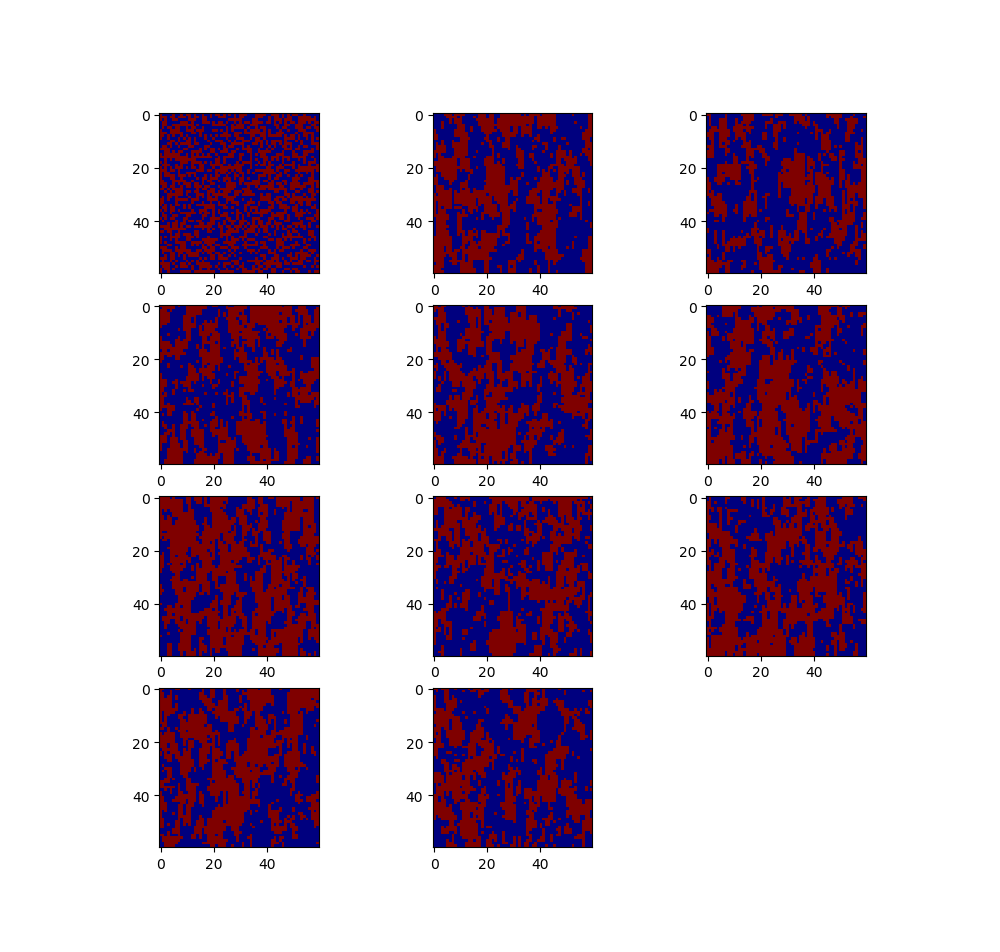
\includegraphics[width=.8\linewidth]{myq82.png}
			\label{82my}
			\caption{Gibbs sampling method, standard}
		\end{subfigure}%
		\begin{subfigure}{.5\textwidth}
			\centering
			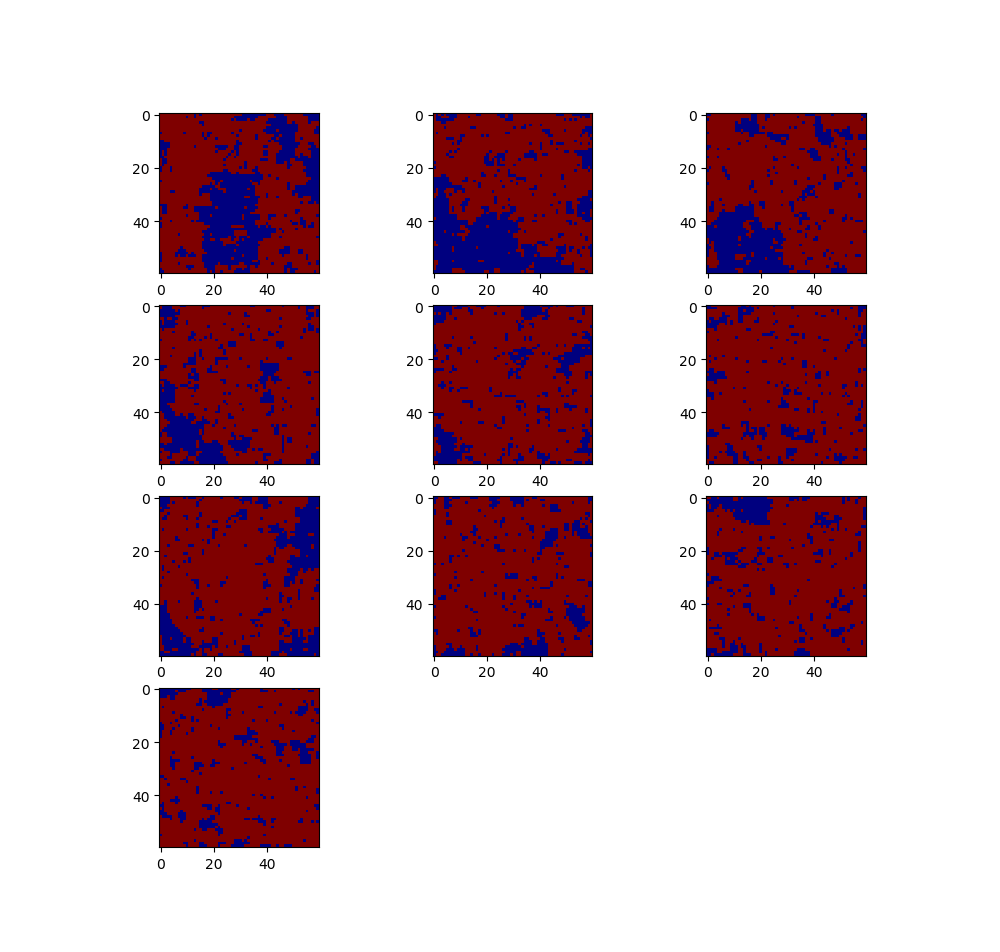
\includegraphics[width=.8\linewidth]{hisq82.png}
			\label{82his}
			\caption{block gibbs sampling}
		\end{subfigure}
		\label{82}
	\end{figure}
	Clearly, it appears that block gibbs sampling mixes much faster than our node by node sampler. It would appear that the initial state, for the block gibbs sampler, is forgotten within the first 5000 iterations. Meanwhile, it seems to be taking quite a bit longer than our standard sampler.
\end{section}

\begin{section}{9.1}
	\subsection{a}
	We have $\mu(x) = \frac{1}{Z_G}\exp(\tilde{\epsilon}\Sigma_{i,j\in E_l}x_ix_j+\theta_v\Sigma_{i\in V_l}x_i)$
	\\
	We can then begin to simplify $F_{MF}(b) = E_b[\log(\psi_{tot}(x))] - \Sigma_i\Sigma_{x_i}b_i(x_i)\log(b_i(x_i))$\\
	 $= F_{MF}(b_v) = E_{b_v}[\log(\psi_{tot}(x))] - \Sigma_i\Sigma_{x_i}b_v(x_i)\log(b_v(x_i)) \\ = 
	 E_{b_v}[\tilde{\epsilon}\Sigma_{i,j\in E_l}x_ix_j+\theta_v\Sigma_{i\in V_l}x_i] - \Sigma_i(b_v(+1)\log(b_v(+1)) - b_v(-1)\log(b_v(-1)))\\
	  = \tilde{\epsilon}\Sigma_{i,j\in E_l}E[x_ix_j]+\theta_v\Sigma_{i\in V_l}E[x_i] - l^2(b_v(+1)\log(b_v(+1)) - b_v(-1)\log(b_v(-1))) \\
	   = \tilde{\epsilon}\Sigma_{i,j\in E_l}(b_v(1)-b_v(-1))^2+\theta_v\Sigma_{i\in V_l}(b_v(1)-b_v(-1))- l^2(b_v(+1)\log(b_v(+1)) - b_v(-1)\log(b_v(-1)))\\
	   = 2l^2\tilde{\epsilon}a^2 + \theta_vl^2(a)- l^2(b_v(+1)\log(b_v(+1)) - b_v(-1)\log(b_v(-1)))$
	   \\
	   As a note, the above we were able to make these simplifications due to the independence we assume between beliefs (which we usually dont have). This lets us plug in and simplify many of these sums with a nice closed form depending on the size of our grid / torus. For example, we can replace the sum over all edges with $2n^2-2n+2n=2n^2$ which accounts for the modulo connections in our graph.
	   \\
	   To simplify this further, we can use the following identity $b_v(1)+b_v(-1) = 1$ and $b_v(1)-b_v(-1) = a$ to get $b_v(1) = \frac{1+a}{2}$ and $b_v(-1) = \frac{1-a}{2}$ 
	   \\
	   Plugging this in we get 
	   $ F_{MF}(a) = 2l^2\tilde{\epsilon}a^2 + \theta_vl^2(a)- l^2(\frac{1+a}{2}\log(\frac{1+a}{2}) - \frac{1-a}{2}\log(\frac{1-a}{2}))$
	   \\
	  Plotting we get the following
	  \begin{figure}[H]
	  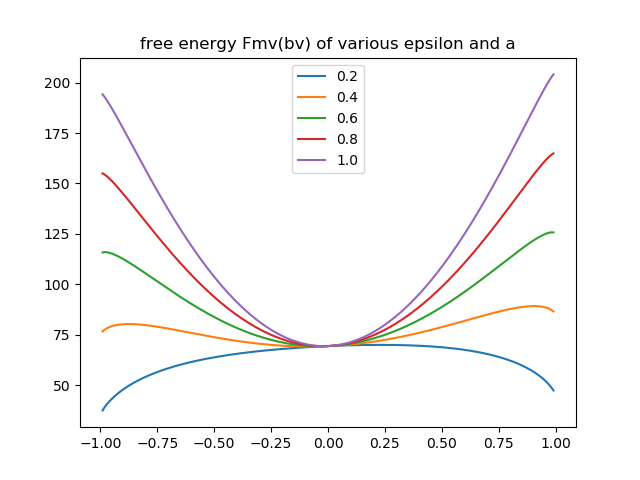
\includegraphics[width=0.7\textwidth]{myq91a1.png}
	  \caption{values of our energy function}
  \end{figure}
To get the maximal value for $b_v(1)$ we will take the gradient of $ F_{MF}(a)$ with respect to $a$ and substitute for our $b_v(1)$ at the end and solve.
\\
$\frac{\partial F}{\partial a} = 4l^2\tilde{\epsilon}a+\theta_vl^2 - \frac{l^2}{2}(\log(1-a)+\log(1+a)+2-\log(4))$
\\
In the appendix you can find the steps done to calculate this. Unfortunately this is only available in written form due to time constraints.
\\
We can then use the fact that $2b_v(1)-1= a$ to substitute to get $\frac{\partial F}{\partial a} = 4l^2\tilde{\epsilon}(2b_v(1)-1)+\theta_vl^2 - \frac{l^2}{2}(\log(1-2b_v(1)+1)+\log(1+2b_v(1)-1)+2-\log(4))$
\\
Using simulation, I was able to solve for the maximal values of F
\begin{figure}[H]
	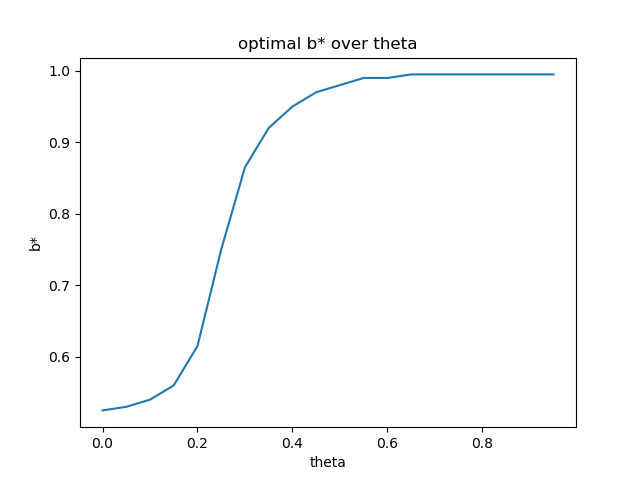
\includegraphics[width=0.7\textwidth]{optimalb.png}
	\caption{values of $b_v$ where the derivative is zero over increasing epsilon 0 to 1}
\end{figure}
Plugging this back into the previously defined $F_{MF}$ we get the maximal values.
\begin{figure}[H]
	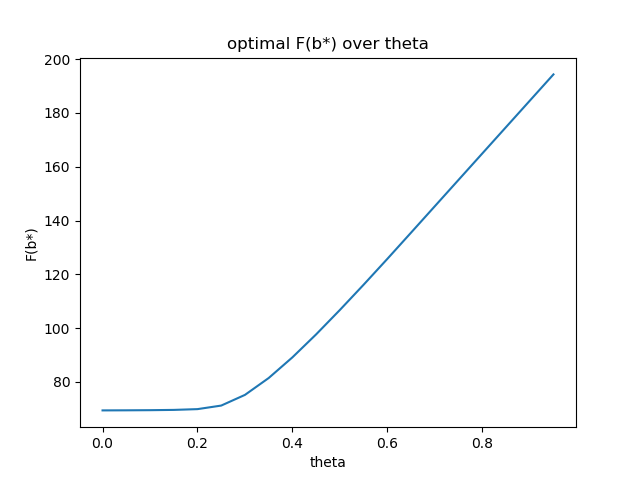
\includegraphics[width=0.7\textwidth]{optimalEnergys.png}
	\caption{max $F_{MF}$ over epsilon 0 to 1}
\end{figure}
	\subsection{b}
	$F(b_v,b_e)=\Sigma_{i,j\in E}E_{b_e}[\log(\psi_{i,j}(x_i,x_j))]+\Sigma_{i\in V}E_{b_v}[\log\psi_i(x_i)]-\Sigma_{i,j\in E}\Sigma_{x_i,x_j}b_e(x_i,x_j)\log(b_e(x_i,x_j))-\Sigma_{i\in V}(1-\deg(i))\Sigma_{x_i}b_{v}(x_i)\log(b_v(x_i)) $
	\\
	\\$= 2N(b_e(1,1)+b_e(-1,-1)-2b_e(1,-1))+N(b_v(1)-b_v(-1))-2N(b_e(1,1)\log(b_e(1,1))+2b_e(1,-1)\log(b_e(1,-1))+b_e(-1,-1)\log(b_e(-1,-1)))-N*3(b_{v}(1)\log(b_v(1))+b_{v}(-1)\log(b_v(-1)))$ We get this by the assumptions made in this problem on our beliefs as well as the symmetry of $b_e$. Also, let $N=l^2$, and we know the number of edges for our torus to be $2l^2$ and the number of vertices to be $l^2$ for obvious reasons.
	\\
	$\frac{\partial L}{\partial b_v(x_i)}=\text{remainder of }F(b_v,b_e)-\Sigma_{i\in V}(1-\deg(i))\Sigma_{x_i}b_{v}(x_i)\log(b_v(x_i))-1+0+0$ As we lost both $\lambda_2$ and $C$ \\
	If I have time I will work on this derivative later. For now im sorry :/ Look to the identity done below for the remainder of my efforts on this HW assignment.
	\\
	\\
	WTS. $\tanh(\theta_e)\tanh(w)=\tanh(\frac{1}{3}(w-\theta_v))$ From before we have $\frac{e^{\theta_e+w}+e^{-\theta_e-w}}{e^{-\theta_e+w}+e^{\theta_e-w}} = e^{-(2/3)\theta_v + (2/3)w}$. Using the equality provided, and having $a = w$ and $b=\theta_e$ we get $2*\frac{1}{2}\log(\frac{e^{\theta_e+w}+e^{-\theta_e-w}}{e^{-\theta_e+w}+e^{\theta_e-w}}) = 2*atanh(\tanh(w)\tanh(\theta_e)) = -(2/3)\theta_v + (2/3)w \rightarrow atanh(\tanh(w)\tanh(\theta_e)) = (1/3)(w-\theta_v) \rightarrow \tanh(w)\tanh(\theta_e) = \tanh((1/3)(w-\theta_v) ) \square$
\end{section}

\begin{section}{Appendix}
	All code can be found here: https://github.com/bogyshi/CSE515/tree/master/HW/hw3
	\\
	code for question 8.2 is in q82.py and the ising\_gibbs\_comb.py files
	\\
	code for question 9.1 is in q91a.py
	\\
	derivation for 9.1a is here
	\begin{figure}[H]
		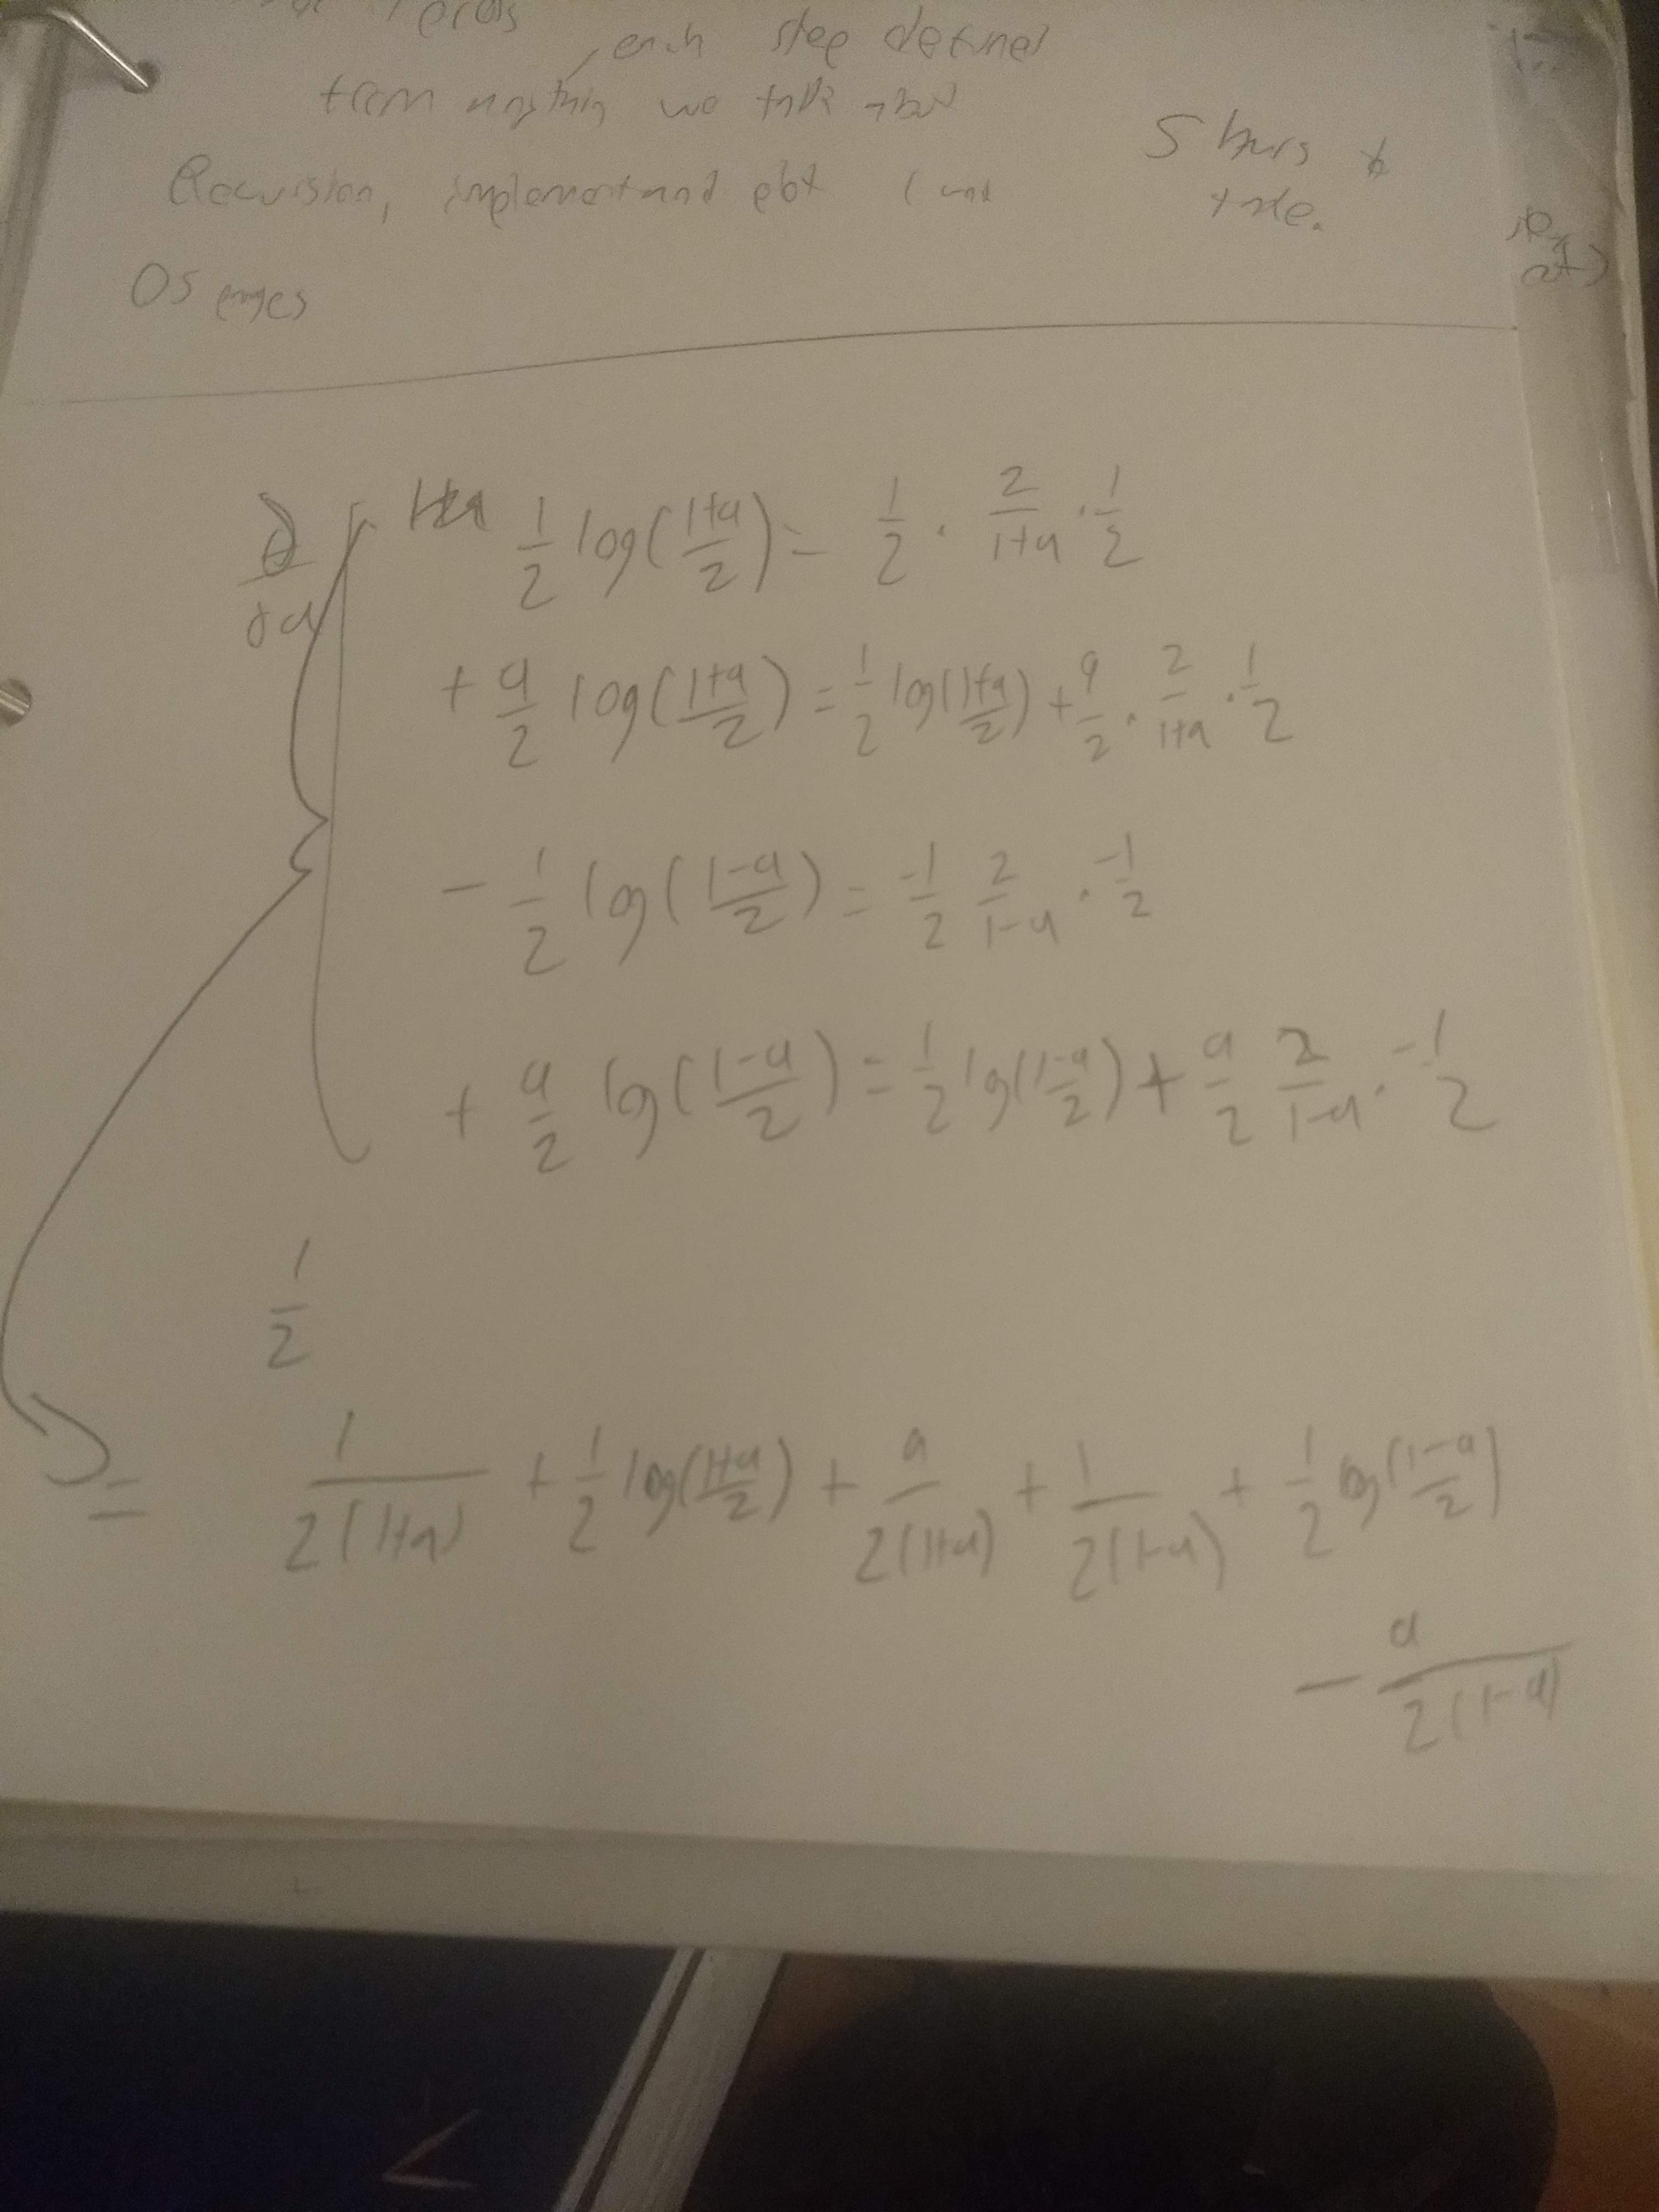
\includegraphics[width=0.7\textwidth]{derivation.jpg}
		\caption{derivation for for F with respect to a}
	\end{figure}
\end{section}

\end{document}

%	\rightarrow \mu(\sigma_j) = \frac{1}{\Sigma_{j-i}\exp(\Sigma_{j,i}w_{i,\sigma(j)})N!}\\
%\ge \frac{1}{\Sigma_{j-i}\exp(\Sigma_{i}w^*)N!}\text{ with w* equal to max of }w_{i,j}\\
%= \frac{1}{\Sigma_{j-i}\exp(Nw^*)N!}\\
%\exp(\Sigma_{i}w_{i,\sigma(i)})\ge \exp(\Sigma_{i}w^*) \text{ with w* equal to max of }w_{i,j}\\
%\rightarrow \exp(\Sigma_{i}w_{i,\sigma(i)})\ge \exp(Nw*)\\
%\rightarrow \frac{1}{Z}\exp(\Sigma_{i}w_{i,\sigma(i)})I(\sigma = \text{perfect matching}) \ge  %\exp(Nw*)
